\subsection{Arquitetura}\label{subsec:arquitetura}

A Arquitetura Geral do Sistema possui 5 grandes m�dulos: Interface Gr�fica, Navega��o, Localiza��o, Sensores e Motores, como pode ser observado na figura \ref{arquitetura:global} abaixo. O m�dulo de Navega��o pode ser dividido em Planejamento, Execu��o e Camada Reativa.
 
\begin{figure}[h]%
\begin{center}
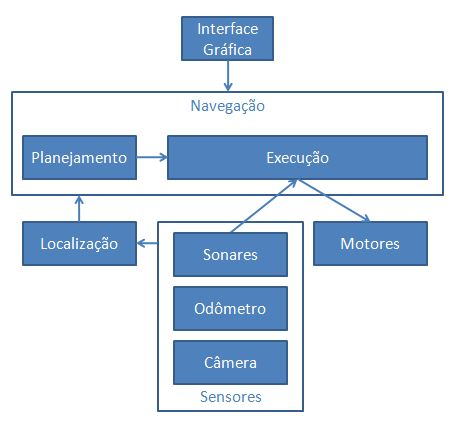
\includegraphics[width=.5\columnwidth]{imagens/arquiteturaGeral.jpg}
\caption{Arquitetura do Sistema completo.}%
\label{arquitetura:global}%
\end{center}
\end{figure}

A Interface Gr�fica apresenta ao usu�rio os poss�veis destinos do rob� e repassa a escolha do usu�rio ao subm�dulo Planejamento, dentro do m�dulo de Navega��o. O Planejamento processa continuamente obtendo os dados do M�dulo de Localiza��o at� chegar ao destino final desejado.

Os Sensores (Sonares, Od�metro e Cam�ra) fornecem as informa��es necess�rias para o M�dulo de Localiza��o estimar sua postura (i.e, coordenadas x, y e \theta). A cada itera��o do m�dulo de Planejamento, ele cria um plano de execu��o, que � passado � Camada Reativa. A Camada Reativa tem a fun��o de evitar colis�es e pode seguir ou n�o o plano de execu��o, baseada na informa��o que os sensores, mais especificamente os Sonares, fornecem.

Por fim, a Camada Reativa envia o comando para os Motores do SAURON.